\subsubsection{Actividad 2 lab 2}
%*********************

\begin{frame}{Actvidad 2 lab 2}
\begin{figure}[H]
\begin{flushleft}
Objetivos:
\end{flushleft}
\begin{flushleft}
-Dar a conocer a lector la distribución  de los diferentes tipos de ruido y sus propiedades.
\end{flushleft}
\begin{flushleft}
-Relacionar las funciones de densidad con cada uno de los diferentes ruidos que aparecen en el modulo noise source.
\end{flushleft}
\begin{flushleft}
-Mediante una breve configuración al lab 2 compare y evidencie que lo anterior se cumpla.
\end{flushleft}

\begin{center}
\centering
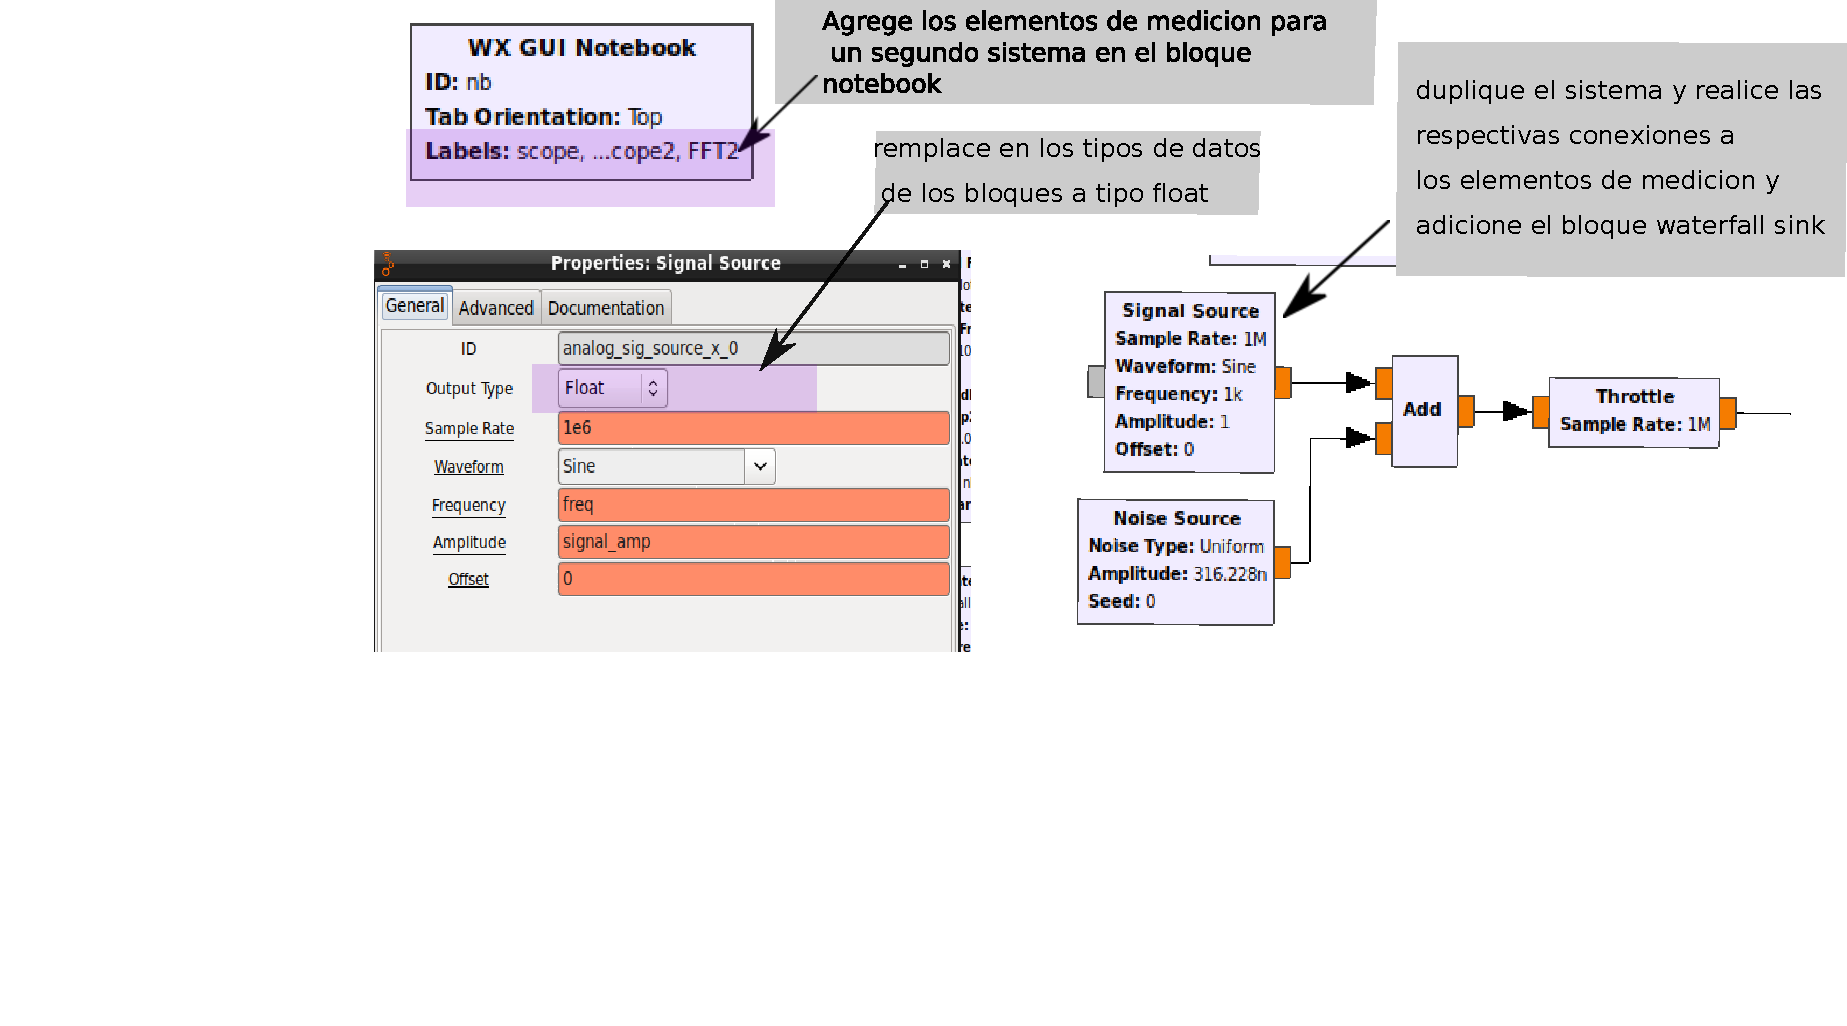
\includegraphics[width=\textwidth, height=0.58\textwidth]{parte1/lab2/pdf/lab2_18.pdf}
\end{center}
\end{figure}
\end{frame}
%--------------------------------
